\documentclass[a4paper,12pt,twoside,openany]{report}
%
% Wzorzec pracy dyplomowej
% J. Starzynski (jstar@iem.pw.edu.pl) na podstawie pracy dyplomowej
% mgr. inż. Błażeja Wincenciaka
% Wersja 0.1 - 8 października 2016
%
\usepackage{polski}
\usepackage{helvet}
\usepackage[T1]{fontenc}
\usepackage{anyfontsize}
\usepackage[utf8]{inputenc}
\usepackage[pdftex]{graphicx}
\usepackage{tabularx}
\usepackage{array}
\usepackage[polish]{babel}
\usepackage{subfigure}
\usepackage{amsfonts}
\usepackage{verbatim}
\usepackage{indentfirst}
\usepackage[pdftex]{hyperref}
\usepackage{listings}
\lstset{aboveskip=20pt,belowskip=20pt}
\usepackage{ucs}
\usepackage[figuresright]{rotating}
\lstset{frame=tb,
		language=Java,
		breaklines=true,
		showstringspaces=false,
		columns=flexible,
		numbers=none,
		tabsize=3,
		inputencoding=utf8x, 
		extendedchars=\true,
		literate={ą}{{\k{a}}}1
		{Ą}{{\k{A}}}1
		{ę}{{\k{e}}}1
		{Ę}{{\k{E}}}1
		{ó}{{\'o}}1
		{Ó}{{\'O}}1
		{ś}{{\'s}}1
		{Ś}{{\'S}}1
		{ł}{{\l{}}}1
		{Ł}{{\L{}}}1
		{ż}{{\.z}}1
		{Ż}{{\.Z}}1
		{ź}{{\'z}}1
		{Ź}{{\'Z}}1
		{ć}{{\'c}}1
		{Ć}{{\'C}}1
		{ń}{{\'n}}1
		{Ń}{{\'N}}1
	}  


% rozmaite polecenia pomocnicze
% gdzie rysunki?
\newcommand{\ImgPath}{.}

% oznaczenie rzeczy do zrobienia/poprawienia
\newcommand{\TODO}{\textbf{TODO}}


% wyroznienie slow kluczowych
\newcommand{\tech}{\texttt}

% na oprawe (1.0cm - 0.7cm)*2 = 0.6cm
% na oprawe (1.1cm - 0.7cm)*2 = 0.8cm
%  oddsidemargin lewy margines na nieparzystych stronach
% evensidemargin lewy margines na parzystych stronach
\def\oprawa{1.05cm}
\addtolength{\oddsidemargin}{\oprawa}
\addtolength{\evensidemargin}{-\oprawa}

% table span multirows
\usepackage{multirow}
\usepackage{enumitem}	% enumitem.pdf
\setlist{listparindent=\parindent, parsep=\parskip} % potrzebuje enumitem

%%%%%%%%%%%%%%% Dodatkowe Pakiety %%%%%%%%%%%%%%%%%
\usepackage{prmag2017}   % definiuje komendy opieku,nrindeksu, rodzaj pracy, ...


%%%%%%%%%%%%%%% Strona Tytułowa %%%%%%%%%%%%%%%%%
% To trzeba wypelnic swoimi danymi
\title{Implementacja portalu do grywalizacji z użyciem platformy SPRING i bazy danych Oracle}

% autor
\author{Jacek Kozieja}
\nrindeksu{261053}

% jeśli wykonawca jest tylko jeden, to usuwamy poniższe polecenia


\opiekun{dr inż. Jacek Korytkowski}
 % opcjonalnie
\terminwykonania{16 maja 2017} % data na oświadczeniu o samodzielności
\rok{2017}


% Podziekowanie - opcjonalne
\podziekowania{\noindent
{\Large Podziękowania}
\bigskip

Dziękujemy bardzo serdecznie wszystkim, a w szczególności Rodzinom i~Unii Europejskiej...

\bigskip

{\raggedleft
Zdolny Student i Pracowity Kolega

}

}

% To sa domyslne wartosci
% - mozna je zmienic, jesli praca jest pisana gdzie indziej niz w ZETiIS
% - mozna je wyrzucic jesli praca jest pisana w ZETiIS
%\miasto{Warszawa}
%\uczelnia{POLITECHNIKA WARSZAWSKA}
%\wydzial{WYDZIAŁ ELEKTRYCZNY}
%\instytut{INSTYTUT ELEKTROTECHNIKI TEORETYCZNEJ\linebreak[1] I~SYSTEMÓW INFORMACYJNO-POMIAROWYCH}
% \zaklad{ZAKŁAD ELEKTROTECHNIKI TEORETYCZNEJ\linebreak[1] I~INFORMATYKI STOSOWANEJ}
%\kierunekstudiow{INFORMATYKA}

% domyslnie praca jest inzynierska, ale po odkomentowaniu ponizszej linii zrobi sie magisterska
%\pracamagisterska
%%% koniec od P.W

\opinie{%
  \newpage
\begin{center}
 {\large\bf  Opinia} \\
o pracy dyplomowej magisterskiej wykonanej przez dyplomanta\\
{\bf Zdolnego Studenta i Pracowitego Kolegę} \\
 Wydział Elektryczny, kierunek Informatyka,  Politechnika Warszawska\\
Temat pracy\\
\textit{\bf
TYTUŁ PRACY DYPLOMOWEJ
}\\
\end{center}
\medskip
\noindent
Promotor: {\bf dr inż. Miły Opiekun}\\
Ocena pracy dyplomowej: {\bf bardzo dobry}

\medskip

\centerline{\bf Treść opinii}
   Celem pracy dyplomowej panów dolnego Studenta i Pracowitego Kolegi  było
opracowanie systemu pozwalającego symulować  i opartego o oprogramowanie o
otwartych źródłach (ang. Open Source). Jak piszą Dyplomanci, starali się opracować
system, który łatwo będzie dostosować do zmieniających się dynamicznie wymagań,
będzie miał niewielkie wymagania sprzętowe i umożliwiał dalszą łatwą rozbudowę oraz
dostosowanie go do potrzeb.
Przedstawiona do recenzji praca składa się z krótkiego wstępu jasno i
wyczerpująco opisującego oraz uzasadniającego cel pracy, trzech rozdziałów (2-4)
zawierających opis istniejących podobnych
rozwiązań, komponentów rozpatrywanychjako kandydaci do
tworzonego systemu i wreszcie zagadnień wydajności wirtualnych
rozwiązań. Piąty rozdział to opis przygotowanego przez
Dyplomantów środowiska obejmujący opis konfiguracji
środowiska oraz przykładowe ćwiczenia laboratoryjne. Ostatni
rozdział pracy to opis możliwości dalszego
rozwoju projektu. W ramach przygotowania pracy Dyplomanci zebrali i przedstawili w
bardzo przejrzysty sposób duży zasób informacji, co świadczy o dobrej orientacji
w nowoczesnej i ciągle intensywnie rozwijanej tematyce stanowiącej
zakres pracy i o umiejętności przejrzystego przedstawienia tych
wyników. Praca zawiera dwa dodatki, z których pierwszy obejmuje wyniki
eksperymentów i badań nad wydajnością, a drugi to źródła
skryptów budujących środowisko.

 Dyplomanci dość
dobrze zrealizowali postawione przed nimi zadanie,
wykazali się więc umiejętnością zastosowania w praktyce wiedzy
przedstawionej w rozdziałach 2-4.  Uważam, że cele postawione w założeniach pracy zostały pomyślnie
zrealizowane. Proponuję ocenę bardzo dobrą (5).

\vskip 1cm
{
\raggedleft
(data, podpis)\kern1cm

}
  \newpage
  \newpage
\begin{center}
 {\large\bf  Recenzja } \\
pracy dyplomowej magisterskiej wykonanej przez dyplomanta\\
{\bf Zdolnego Studenta i Pracowitego Kolegę} \\
 Wydział Elektryczny, kierunek Informatyka,  Politechnika Warszawska\\
Temat pracy\\
\textit{\bf
TYTUŁ PRACY DYPLOMOWEJ
}\\
\end{center}
\medskip
\noindent
Recenzent: {\bf prof. nzw. dr hab. inż. Jan Surowy}\\
Ocena pracy dyplomowej: {\bf bardzo dobry}
\medskip


\centerline{\bf Treść recenzji}
   Celem pracy dyplomowej panów dolnego Studenta i Pracowitego Kolegi  było
opracowanie systemu pozwalającego symulować  i opartego o oprogramowanie o
otwartych źródłach (ang. Open Source). Jak piszą Dyplomanci, starali się opracować
system, który łatwo będzie dostosować do zmieniających się dynamicznie wymagań,
będzie miał niewielkie wymagania sprzętowe i umożliwiał dalszą łatwą rozbudowę oraz
dostosowanie go do potrzeb.
Przedstawiona do recenzji praca składa się z krótkiego wstępu jasno i
wyczerpująco opisującego oraz uzasadniającego cel pracy, trzech rozdziałów (2-4)
zawierających bardzo solidny i przejrzysty opis: istniejących podobnych
rozwiązań (rozdz. 2), komponentów rozpatrywanychjako kandydaci do
tworzonego systemu (rozdz. 3) i wreszcie zagadnień wydajności wirtualnych
rozwiązań, zwłaszcza w kontekście współpracy  kilku elementów
 sieci (rozdział 4). Piąty rozdział to opis przygotowanego przez
Dyplomantów środowiska obejmujący opis konfiguracji
środowiska oraz przykładowe ćwiczenia laboratoryjne (5 ćwiczeń). Ostatni, szósty
rozdział pracy to krótkie zakończenie, które wylicza także możliwości dalszego
rozwoju projektu. W ramach przygotowania pracy Dyplomanci zebrali i przedstawili w
bardzo przejrzysty sposób duży zasób informacji o narzędziach, Rozdziały 2, 3 i 4 świadczą o dobrej orientacji
w nowoczesnej i ciągle intensywnie rozwijanej tematyce stanowiącej
zakres pracy i o umiejętności syntetycznego, przejrzystego przedstawienia tych
wyników. Drobne  mankamenty tej części pracy to zbyt skrótowe omawianie
niektórych zagadnień technicznych, zakładające dużą początkową wiedzę czytelnika
i dość niestaranne podejście do powołań na źródła.
Utrudnia to w pewnym stopniu czytanie pracy i zmniejsza jej wartość dydaktyczną
(a ta zdaje się być jednym z celów Autorów), ale jest zrekompensowane zawartością
merytoryczną. Praca zawiera dwa dodatki, z których pierwszy obejmuje wyniki
eksperymentów i badań nad wydajnością, a drugi to źródła
skryptów budujących środowisko. Praca
zawiera niestety dość dużą liczbę drobnych błędów redakcyjnych, ale nie wpływają
one w sposób istotny na na jej czytelność i wartość. W całej pracy przewijają
się samodzielne, zdecydowane wnioski Autorów, które są wynikiem własnych i
oryginalnych badań.  Rozdział 5 i dodatki pracy przekonują mnie, że Dyplomanci dość
dobrze zrealizowali postawione przed nimi zadanie. Pozwala to stwierdzić, że
wykazali się więc także umiejętnością zastosowania w praktyce wiedzy
przedstawionej w rozdziałach 2-4. Kończący pracę rozdział szósty świadczy o
dużym (ale moim zdaniem uzasadnionym) poczuciu własnej wartości i jest
świadectwem własnego, oryginalnego spojrzenia na tematykę przedstawioną w pracy
dyplomowej. Uważam, że cele postawione w założeniach pracy zostały pomyślnie
zrealizowane. Proponuję ocenę bardzo dobrą (5).

\vskip 1cm
{
\raggedleft
(data, podpis)\kern1cm

}
}

\streszczenia{
  \newpage
\begin{center}
\large \bf
Implementacja portalu do grywalizacji z użyciem platformy SPRING i bazy danych Oracle
\end{center}

\section*{Streszczenie}
Praca składa się z krótkiego wstępu opisującego cel oraz strukturę wykonanego projektu, trzech rozdziałów
zawierających opis wykorzystanych technologii (szkielet Angular, szkielet Spring i baza danych Oracle) i przykłady ich zastosowań w projekcie. Czwarty rozdział to opis zagadnień związanych z bezpieczeństwem współczesnych aplikacji internetowych. Rozdział piąty przedstawia wdrożenie aplikacji do chmury obliczeniowej. W rozdziale szóstym można zapoznać się z działaniem aplikacji w praktyce - zawiera on opis funkcjonalności z perspektywy Użytkownika końcowego. Ostatni rozdział to wnioski, dotyczące wydajności i sposobów tworzenia aplikacji.

\bigskip
{\noindent\bf Słowa kluczowe:} Spring, Angular, Oracle

\vskip 2cm


\begin{center}
\large \bf
Implementation of gamification web portal based on SPRING framework and Oracle databse
\end{center}

\section*{Abstract}
This thesis consists of a short introduction that describes goal and structure of a project. Next three chapters depict used technologies (Angular framework, Spring framework and Oracle database) and their use in the project. Fourth chapter is a description of security topics related to modern web applications. Fifth chapter shows cloud migration of a system. The sixth chapter includes description of funcionalities from an end-user perspective - it shows a practical use of the application. The last one is a conclusion about overall performance and approach to application development.

\bigskip
{\noindent\bf Keywords:} Spring, Angular, Oracle

\vfill
}

\begin{document}
\maketitle
%-----------------
% Wstęp
%-----------------
\chapter{Wstęp}
Celem pracy było stworzenie aplikacji internetowej, motywującej grupy ludzi do wspólnej pracy poprzez system wyzwań i nagród. Należy jednak pamiętać że o ile aplikacja pomaga zarządzać zadaniami, prowadzić ranking i kontrolować rozwój użytkowników, o tyle weryfikacja wykonanych zadań czy przyznawanie fizycznych nagród pozostaje obowiązkiem administratora. Stworzone rozwiązanie było także pretekstem do zbadania współczesnych technologii wytwarzania aplikacji internetowych, opisanych w dalszej części pracy.
\section{Grywalizacja}
	Grywalizacja, gryfikacja lub gamifikacja, to zgodnie z definicją \cite{Wikipedia} "Wykorzystanie mechaniki znanej np. z gier fabularnych i komputerowych, do modyfikowania zachowań ludzi w sytuacjach życia codziennego, w celu zwiększenia zaangażowania ludzi." Ta szeroka definicja obejmuje rozwiązania stosowane w marketingu, zarządzaniu projektami jak i edukacji.
	\section{Projekt}
	Plany stworzenia aplikacji ,,Gamify'' przybliżyć mogą poniższe przykładowe Przypadki Użycia:\\
	UC Użytkownika:\\
	Wykonanie Zadania
	\begin{enumerate}
		\item Użytkownik loguje się do Systemu.
		\item Użytkownik wybiera opcję ,,Wykonaj Zadanie'' (Ścieżka alternatywna):
		\begin{enumerate}
		\item Użytkownik skanuje kod QR
		\item System dodaje zadanie i punkty Użytkownikowi
		\end{enumerate}
		\item System wyświetla formularz wykonania Zadania.
		\item Użytkownik wpisuje numer Zadania.
		\item System dodaje zadanie i punkty Użytkownikowi
	\end{enumerate}
	Przejrzenie tabeli Rankingu
	\begin{enumerate}
		\item Użytkownik loguje się do Systemu.
		\item Użytkownik wybiera opcję ,,Ranking''.
		\item System wyświetla tabelę Użytkowników.
		\item Użytkownik wybiera sortowanie malejąco, po Punktach.
		\item System wyświela posortowaną listę.
	\end{enumerate}
	UC Administratora:\\
	Dodanie nowego Zadania
	\begin{enumerate}
		\item Administrator loguje się do systemu
		\item Administrator wybiera opcję ,,Dodaj Zadanie''
		\item System wyświetla formularz dodania Zadania.
		\item Administrator podaje opis, datę końcową i punkty Zadania.
		\item System generuje numer Zadania i zapisuje je.
	\end{enumerate}
	Przynanie Odznaki Użytkownikom
	\begin{enumerate}
		\item Administrator loguje się do Systemu.
		\item Administrator wybiera opcję ,,Odznaki''.
		\item System wyświetla okno edycji Odznak.
		\item Administrator wybiera opcję ,,Przyznaj odznakę''
		\item System wybiera okno wyboru Odznaki.
		\item Administrator wybiera Odznakę.
		\item System wyświetla okno wyboru Użytkowników.
		\item Administrator wybiera Użytkowników.
		\item System przyznaje odznakę wybranym Użytkownikom.
	\end{enumerate}
	Diagramy klas na Rysunkach 1.1 i 1.2 opisują strukturę modułu GLogin - oddzielnie dla wnętrza (,,back-end'') i fasady (,,front-end''). Są one reprezentatywne dla całości projektu, zaś stworzenie pełnej dokumentacji uważam za odpowiedni temat dla oddzielnej pracy dyplomowej. Prywatne zmienne posiadające publiczne metody dostępowe zostały przedstawione jako zmienne publiczne. Redukuje to liczbę metod i zwiększa czytelność diagramów.
	\begin{sidewaysfigure}[!htbp]

			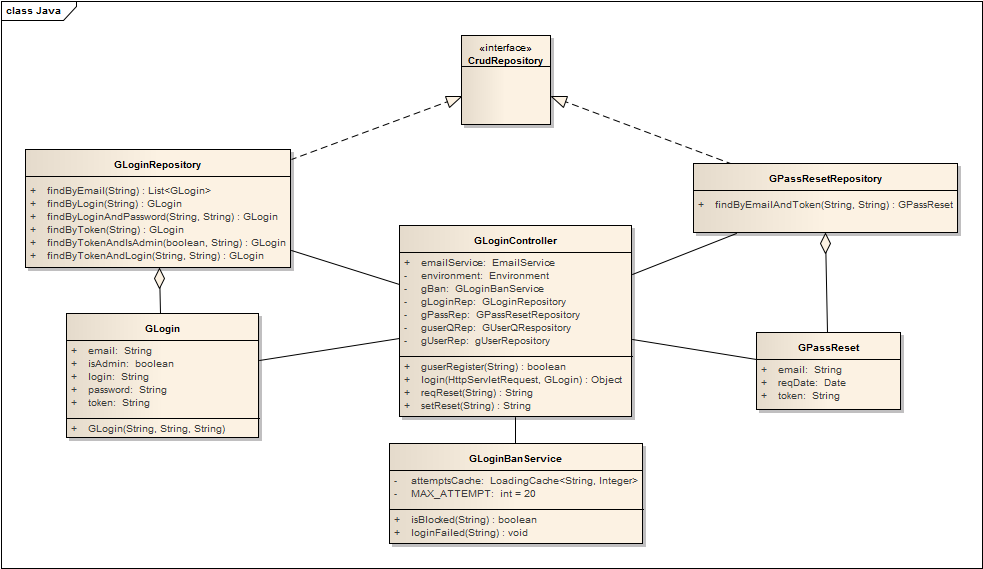
\includegraphics[scale=0.7]{\ImgPath/rys/UML-Java.png}

		\caption{Diagram klas w języku Java.}
		\label{UMLJava}
	\end{sidewaysfigure}
		\begin{sidewaysfigure}[!htbp]

				\includegraphics[scale=0.7]{\ImgPath/rys/UML-TS2.png}

			\caption{Diagram klas w języku TypeScript.}
			\label{UMLTS}
		\end{sidewaysfigure}
\section{Użyte technologie}
Do wykonania aplikacji użyto technologii, przedstawionych na Rysunku 1.3.
	\begin{figure}[!htbp]
		\begin{center}
			\centering
			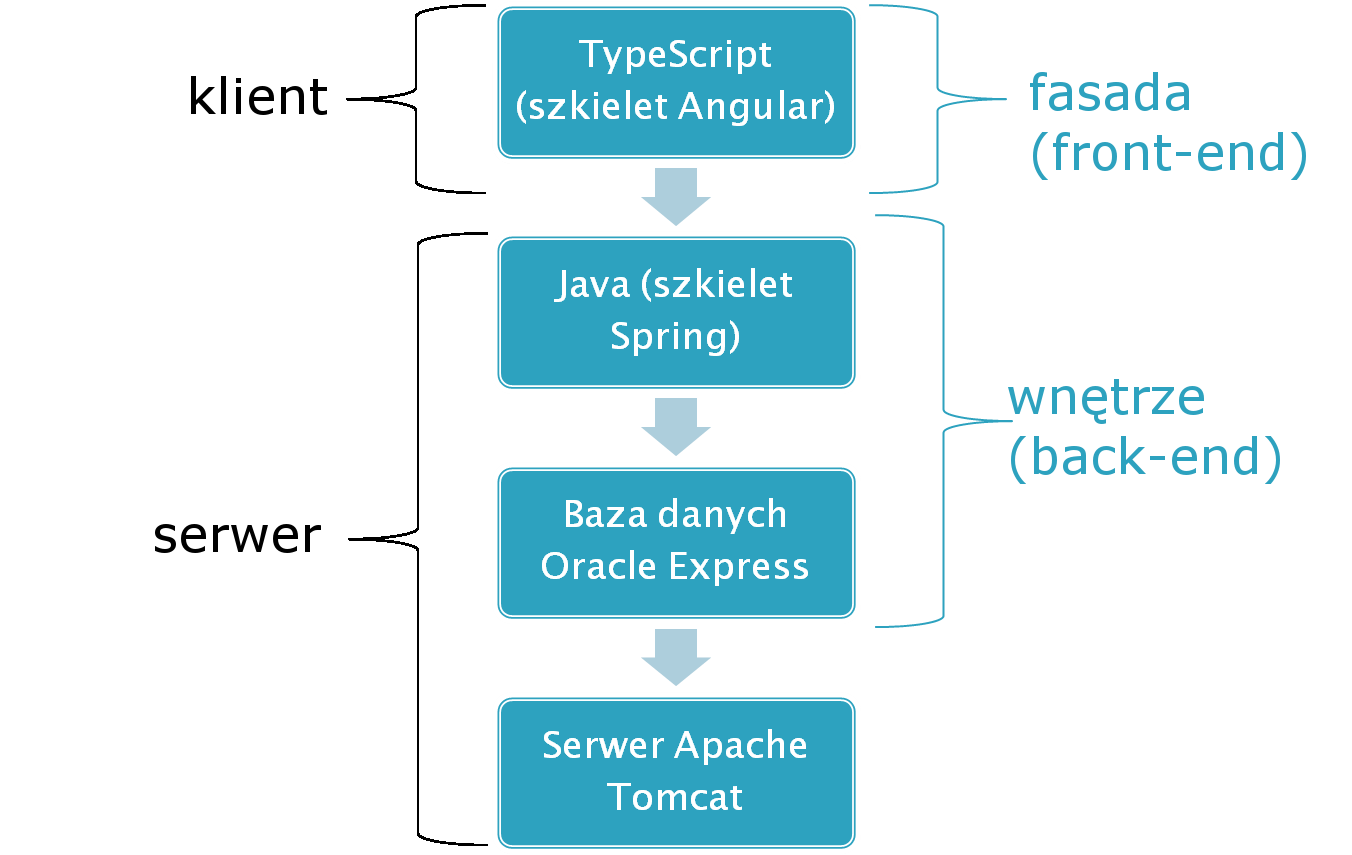
\includegraphics[width=\textwidth]{\ImgPath/rys/technologies.png}
		\end{center}
		\caption{Języki, szkielety i systemy bedące częścią projektu.}
		\label{technologies}
	\end{figure}
Jak widać, aplikacja została wykonana w architekturze Klient-Serwer, opisanej w [LITERATURA]. Fasada oznacza kod wykonywany przez przeglądarkę internetową po stronie Klienta. Warstwa Klienta obsługuje żądania Użytkownika, wysyła zapytania do Serwera i prezentuje odpowiedzi Użytkownikowi. Wnętrze oznacza kod wykonywany po stronie Serwera. Serwer nasłuchuje żądań Klienta, wykonuje logikę biznesową związaną z danym żadaniem i wysyła odpowiedź do Klienta. Z usług jednego Serwera może korzystać wiele instancji Klientów. Obydwie składowe wykorzystują inne technologie, opisane szerzej w kolejnych rozdziałach.
\section{Wzorzec MVC}
Złożoność współczesnych aplikacji (w tym internetowych), wymusza wykorzystanie odpowiednich wzorców (projektowych, architektonicznych). Narzucają one sprawdzoną formę, która pozwala zapanować nad rozbudowanym kodem. W tworzonej aplikacji, zdecydowano się na wykorzystanie wzorca MVC. Jest on szeroko opisywany w literaturze, chociażby w [LITERATURA], oraz jest wykorzystywany przez wybrane szkielety aplikacji. MVC to wzorzec architektoniczny służący do organizowania struktury systemów interaktywnych. Składa się on z trzech części:
	\begin{enumerate}
		\item Model - reprezentuje dane i wykonuje logikę biznesową.
		\item Widok - wyświetla dane pobrane z Modelu.
		\item Kontroler - reaguje na dane wejściowe użytkownika. Przesyła żądania wykonania logiki biznesowej do Modelu i zmian Widoku. 
	\end{enumerate}
Zarówno Angular jak i Spring samodzielnie realizują wzorzec MVC. Jednak gdy połączymy te dwie technologie, sytuacja zmienia się. Warstwa kontrolera przeniesiona jest do Angulara i jest wykonywana przez przeglądarkę. To samo samo dzieje się z warstwą widoku. Po stronie serwerowej Springa pozostaje warstwa modelu. Ten rozdział powoduje że potrzebny jest odpowiedni sposób komunikacji Klient-Serwer. Nazywa się on REST API. Skróty te oznaczają Representational State Transfer i Application Programming Interface. Pierwszy skrót oznacza bezstanową wymianę tekstowych zasobów sieciowych. Przykładem są tu zapytania HTTP GET, POST, PUT, DELETE. Drugi skrót oznacza jednoznacznie zdefiniowany sposób komunikacji między komponentami. W wypadku aplikacji internetowej oznacza to że strona serwerowa odbierając zapytanie HTTP pod danym adresem, powinna zwrócić odpowiedź w postaci XML lub JSON. Przykład zapytania do takiego API i odpowiedzi, znajduje się na Rysunku 1.4.
		\begin{figure}[!htbp]
			\begin{center}
				\centering
				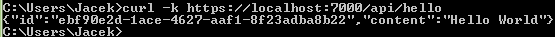
\includegraphics[width=\textwidth]{\ImgPath/rys/testAPI.png}
			\end{center}
			\caption{Zapytanie do API i odpowiedź. Taka komunikacja pozwala wykorzystać tą samą warstwę modelu w kilku różnych aplikacjach.}
			\label{UMLTS}
		\end{figure}
Modułowa struktura projektu jest przedstawiona na Rysunku 1.5. Przedstawia się ona następująco: wewnątrz projektu Springa rezydują obok siebie 3 foldery - z plikami źródłowymi Javy, plikami statycznymi (grafiką) i projektem Angulara. Obydwa języki posiadają moduły główne - tam przechowywane są konfiguracje i najczęściej używane klasy. Każda większa funkcjonalność posiada oddzielny folder. To samo tyczy się aplikacji admina która jest traktowana jako oddzielny moduł. Przedrostek \textit{,,g''} występujący w nazwach klas i modułów podyktowany jest zbieżnoscią nazw takich jak login czy user z natywnymi elementami użytych platform.
		\begin{figure}[!htbp]
			\begin{center}
				\centering
				\includegraphics[width=\textwidth]{\ImgPath/rys/appmodules.png}
			\end{center}
			\caption{Modułowy podział projektu.}
			\label{UMLTS}
		\end{figure}
\chapter{Angular}
Do wytworzenia warstwy klienckiej użyto szkieletu Angular w wersji drugiej. Wybrano go ze względu na ciekawy, rzadko spotykany w aplikacjach internetowych sposób działania. Cały kod jest wczytywany przez przeglądarkę internetową na samym początku korzystania z aplikacji. Skutki takiego rozwiązania są pokazane w Rozdziale \ref{Ending} Wnioski. Szkielet ten jest rozwijany przez firmę Google, która wyznacza trendy współczesnych usług sieciowych. Bez względu na specjalizację i miejsce programisty w stosie technologicznym, warto sie z nim zapoznać. Kto wie kiedy przyjdzie nam pisać logikę biznesową, współpracującą z tym szkieletem.
Szkielet ten wykorzystuje język Typescript. Jest to nadzbiór języka JavaScript i jest do niego kompilowany. Przykłady definicji klas były prezentowane wcześniej, na Rysunku 1.2. Rozwiązania używane w fasadzie aplikacji internetowych są bez wątpienia najszybciej rozwijającym sie elementem stosu technologicznego. Już w momencie pisania pracy moda na Angulara ustępuje modzie na bibliotekę React, rozwijaną przez firmę Facebook. Jako że wnętrze aplikacji działa niezależnie od fasady, nie będzie ona opisywana szerzej w tej pracy. Zainteresowani, mogą zgłębić wiedzę na ten temat, czytając oficjalną dokumentację \cite{Angular}. W przystępny sposób przeprowadza ona użytkownika przez proces tworzenia funkcjonalnej aplikacji i pozwala zaznajomić się z konceptami stojącymi za tym szkieletem.
\chapter{Spring}
Podjęto decyzję by warstwę serwerową napisać z pomocą szkieletu Spring. Wybrano go między innymi ze względu na bogatą dokumentację, mnogość przydatnych modułów i dostępność szybkich sposobów na konfigurację sprawnej aplikacji serwerowej.
Spring to szkielet tworzenia aplikacji (ang. framework) przeznaczony dla Javy Enterprise Edition, czyli serwerowej odmiany tego języka. Powstał jako alternatywa dla oficjalnych standardów serwerowych Javy takich jak Enterprise JavaBeans. Spring nie narzuca jednego modelu programowania. Posiada wiele modułów które są przydatne przy pisaniu aplikacji, jednocześnie będąc całkowicie opcjonalnymi. Znaną cechą Springa LITERATURA jest \textbf{,,odwrócenie sterowania''} (ang. Inversion of Control), czyli wzorzec w którym wykonywaniem programu steruje szkielet a nie kod programisty. To Spring decyduje kiedy wykonać dane akcje. Przykładem odwróconego sterowania jest chociażby \textbf{"wstrzykiwnie zależności"} (ang. Dependency Injection), kiedy to utworzone, zainicjowane obiekty przekazywane są obiektom które ich potrzebują. Obiekty nie tworzą wtedy samodzielnie instancji innych obiektów. Kolejną ważną cechą Springa jest \textbf{,,programowanie aspektowe''} czyli wzorzec w którym rozdziela się fizycznie funkcjonalności i definiuje punkty komunikacji między nimi, dostępne wszędzie tam gdzie są potrzebne.
\section{Metody konfiguracji}
Konfiguracja projektu w Springu może odbywać się na dwa sposoby - przy pomocy plików XML lub adnotacji.Obydwa te podejścia przedstawiono w kursie \cite{Spring2}  Poniższy przykład prezentuje te same ustawienia w obydwu reprezentacjach:\\
\begin{tabular}{|l|l|}
	\hline XML\\ 
	\hline <beans> \\
	<bean id = ''myClass'' \\ class = ''com.koziejaj.MyClass'' />\\
	</beans>\\ \\
	\hline 
\end{tabular} 
\begin{tabular}{|l|l|}
	\hline Adnotacje\\ 
	\hline @Configuration\\
	public class MyClassConfig \{\\
	@Bean \\
	public MyClass myClass()\{\\
	return new MyClass();
	\}
	\}\\
	\hline 
\end{tabular}\\\\\\
Konfiguracja XML odbywa się w oddzielnych plikach, zaś przy pomocy adnotacji - bezpośrednio w kodzie którego dotyczy. Warto wiedzieć że konfiguracja adnotacjami wykonuje się przed XML. W projekcie użyto adnotacji. Wydają się one czytelniejsze, są też kierunkiem w którym zmierza rozwój Springa. Wyjątkiem są pliki z rozszerzeniem \textit{,,.properties''}. Przechowują one stałe wartości, takie jak numer portu serwera, dane uwierzytelniające bazy danych.
\section{Spring Boot}
Brak narzuconych standardów szkieletu aplikacji ma także i swoje wady. Spring wymaga dużej ilości konfiguracji, a także dobrania modułów i bibliotek które będą nam potrzebne. Moduł Spring Boot zawiera wstępną konfigurację i najpotrzebniejsze biblioteki. Jednocześnie umożliwia dostosowanie projektu do specyficznych wymagań. Podczas uruchomienia sprawdza których elementów konfiguracji brakuje i dodaje je zgodnie z posiadaną wiedzą na temat projektu. Moduł ten można uznać za fundament stworzonej aplikacji. Ilość kodu wymaganą do napisania aplikacji serwerowej w ramach Spring Boot przedstawiają poniższe listingi, zgodne z podejściem przedstawionym w \cite{Spring}:

\begin{lstlisting}[label={MVCController}]
package hello;

import org.springframework.web.bind.annotation.RestController;
import org.springframework.web.bind.annotation.RequestMapping;

@RestController
public class HelloController {

	@RequestMapping("/")
	public String index() {
	return "Witaj Swiecie! Pozdrowienia od Spring Boot!\n";
	}
}
\end{lstlisting}
Adnotacja \textit{,,@RestController''} informuje moduł Spring MVC że klasa będzie przystosowana do ubsługi zapytań sieciowych. Adnotacja \textit{,,@RequestMapping(''/'')''} oznacza ścieżkę która spowoduje wywołanie metody.

\begin{lstlisting}
package hello;

import java.util.Arrays;

import org.springframework.boot.CommandLineRunner;
import org.springframework.boot.SpringApplication;
import org.springframework.boot.autoconfigure.SpringBootApplication;
import org.springframework.context.ApplicationContext;
import org.springframework.context.annotation.Bean;

@SpringBootApplication
public class Application {

	public static void main(String[] args) {
		SpringApplication.run(Application.class, args);
	}

	@Bean
	public CommandLineRunner commandLineRunner(ApplicationContext ctx) {
		return args -> {

			System.out.println("Klasy Projektu:");

			String[] beanNames = ctx.getBeanDefinitionNames();
			Arrays.sort(beanNames);
			for (String beanName : beanNames) {
				System.out.println(beanName);
			}

		};
	}

}
\end{lstlisting}
Adnotacja \textit{,,@SpringBootApplication''} jest wygodnym połączeniem kilku innych adnotacji: 
\begin{itemize}
	\item \textit{,,@Configuration''} - oznacza klasę jako źródło metod z adnotacją @Bean, które powinne być dostępne w kontekście aplikacji.
	\item \textit{,,@EnableAutoConfiguration''} - nakazuje Spring Boot dodać do kontekstu aplikacji wszystkie metody \textit{,,@Bean''} na podstawie ścieżki projektu, innych metod \textit{,,@Bean''} i dostępnych konfiguracji.
	\item \textit{,,@ComponentScan''} - skanuje pakiet (w tym przypadku ,,hello'') w poszukiwaniu komponentów, konfiguracji i serwisów.
\end{itemize}
Metoda \textit{,,SpringApplication.run();''} uruchamia aplikację, zaś metoda zwracająca \textit{,,CommandLineRunner''} jest uruchamiana podczas startu. Rysunek 3.1 przedstawia uruchomioną aplikację, zaś Rysunek 3.2 - obsłużenie zapytania.
		\begin{figure}[!htbp]
			\begin{center}
				\centering
				\includegraphics[width=\textwidth]{\ImgPath/rys/helloWorld.png}
			\end{center}
			\caption{Fragment uruchomienia skompilowanego przykładu.}
			\label{UMLTS}
		\end{figure}
				\begin{figure}[!htbp]
					\begin{center}
						\centering
						\includegraphics[width=\textwidth]{\ImgPath/rys/helloWorld2.png}
					\end{center}
					\caption{Zapytanie wysłane do przykładu.}
					\label{UMLTS}
				\end{figure}
				

\section{Maven}
Maven to w narzędzie do zarządzania projektem - jego zależnościami (używanymi bibliotekami) i strukturą (podziałem na moduły). Maven automatyzuje budowę projektu zgodnie z poniższymi krokami \cite{Maven}.
\begin{enumerate}
	\item Validate - walidacja kodu. Sprawdzana jest poprawność kodu źródłowego, umożliwiająca jego kompilację.
	\item Compile - kompilacja, czyli przetworzenie kodu źródłowego na kod bajtowy, wykonywany przez maszynę wirtualną Javy.
	\item Test - wykonanie testów jednostkowych.
	\item Package - budowa pojedynczej paczki wykonywalnej (plik .JAR) lub wykonywanej przez serwer (plik .WAR).
	\item Integration-test - wykonanie testów integracyjnych.
	\item Verify - weryfikacja jakościowa paczki zbudowanej w kroku 4.
	\item Install - instalacja paczki. Oznacza to umieszczenie paczki z kroku 4 w repozytorium lokalnym lub zdalnym.
	\item Deploy - umieszczenie projektu w repozytorium.
\end{enumerate}
				\begin{figure}[!htbp]
					\begin{center}
						\centering
						\includegraphics[width=\textwidth]{\ImgPath/rys/mavencycle.png}
					\end{center}
					\caption{Uproszczony cykl życia projektu Maven.}
					\label{UMLTS}
				\end{figure}
Konfiguracja Maven znajduje sie pliku POM.xml. Poniższy przykład przedstawia skróconą wersję pliku POM stworzonego projektu:

\begin{lstlisting}
<!-- Nagłówek określający używaną wersję -->
<project xmlns="http://maven.apache.org/POM/4.0.0" xmlns:xsi="http://www.w3.org/2001/XMLSchema-instance"
xsi:schemaLocation="http://maven.apache.org/POM/4.0.0 http://maven.apache.org/maven-v4_0_0.xsd">

<!-- Podstawowe informacje na temat projektu -->
<modelVersion>4.0.0</modelVersion>
<groupId>com.koziejaj.client</groupId>
<artifactId>gamify</artifactId>
<packaging>jar</packaging>
<version>0.1-dev</version>
<name>gamify</name>
<url>http://maven.apache.org</url>

<!-- Dziedziczenie po istniejącaym projekcie -->
<parent>
<groupId>org.springframework.boot</groupId>
<artifactId>spring-boot-starter-parent</artifactId>
<version>1.4.2.RELEASE</version>
</parent>

<!-- Zależności - lista bibliotek które należy pobrać -->
<dependencies>
<dependency>
<groupId>org.springframework.boot</groupId>
<artifactId>spring-boot-starter-web</artifactId>
</dependency>
<dependency>
<groupId>org.springframework.boot</groupId>
<artifactId>spring-boot-starter-security</artifactId>
</dependency>
</dependencies>

<!-- Dodatkowe ustawienia -->
<properties>
<java.version>1.8</java.version>
</properties>

</project>

\end{lstlisting}

\section{Przydatne moduły}
Oto lista najważniejszych modułów użytych w projekcie:
\begin{itemize}
	\item Spring MVC - przy pomocy klasy \textit{,,DispatcherServlet''} przekazuje zapytania do odpowiednich kontrolerów, tak jak na pierwszym fragmencie kodu z Podrozdziału \ref{MVCController} Spring Boot. W przypadku wykonanego projektu, jest częścią modułu spring-boot-starter-web.
	\item Spring Data - rozbudowana, wielomodułowa biblioteka, wspierająca warstwę dostępu do danych. Wypiera popularną niegdyś bibliotekę Hibernate. W przypadku Gamify, użyto dwóch modułów:
	\begin{itemize}
		\item JPA - służy do mapowania obiektowo-relacyjnego zgodnie ze standardem JPA. Pobrany jako moduł spring-boot-starter-data-jpa.
		\item REST - Umożliwia tworzenie repozytoriów z automatycznie generowanymi metodami CRUD. Obiekt takiego repozytorium odpowiada tabeli w bazie danych. Mogą być one z łatwością rozbudowane o szczegółowe metody obróbki danych. Przykładowo, metoda 
		\begin{lstlisting}
		GLogin findByLoginAndPassword(String login, String password);
		\end{lstlisting}
		wyszuka użytkowników o określonym loginie i haśle bez potrzeby pisania jakiejkolwiek logiki biznesowej. REST umożliwia wysyłanie zapytań do repozytoriów w sposób analogiczny do kontrolerów (Podrozdział \ref{MVCController}), jednak ta funkcjonalność nie została wykorzystana w projekcie. Moduł pobrany jako: spring-boot-starter-data-rest.
	\end{itemize}
	\item Spring Security - biblioteka zapewniająca bezpieczeństwo aplikacji, szerzej opisana w rozdziale Bezpieczeństwo \ref{Safety}.
\end{itemize}
\section{Implementacja REST API}
Implementacja serwerowej części aplikacji zostanie omówiona na przykładzie modułu panelu Administratora. Ograniczy to analizę do sześciu klas, zorganizowanych podobnie do wcześniejszego Rysunku \ref{UMLJava}.
\subsection{Mapowanie obiektowo - relacyjne}
Klasy omówione w tej sekcji są definicjami tabel bazy danych. Zostały one wytworzone zgodnie z poradnikiem ,,Accessing Data JPA'' \cite{Spring}. Klasa taka odpowiada pojedynczemu rekordowi tabeli i pozwala na jego modyfikację.\\ 
Jedną z funkcjonalności panelu Administratora jest tworzenie i przyznawanie Odznak. Jest to taki wirtualny medal za specjalne zasługi, który Administrator może nadać Użytkownikowi. Instancja takiego medalu musi zawierać dwie informacje - unikatowy login Użytkownika który go posiada i nazwę Odznaki. Nazwa ta odpowiada plikowi graficznemu Odznaki w plikach statycznych projektu.
\begin{lstlisting}
package com.koziejaj.client.GAdmin;


import ...
//Adnotacja oznaczająca klasę odpowiadającą tabeli bazy danych
@Entity
//Adnotacja wczytująca definicję klucza głównego (primary key) - wyjaśnienie w kolejnym listingu
@IdClass(GBId.class)
public class GBadge{

	//Adnotacje klucza głównego
	@Id
	private String login;
	@Id
	private String badge;

	//Konstruktory
	public GBadge() {
	}

	public GBadge(String i, String v) {
	login = i;
	badge = v;
	}

	//Metody dostępowe
	public String getLogin() {
	return login;
	}

	public void setLogin(String login) {
	this.login = login;
	}

	public String getBadge() {
	return badge;
	}

	public void setBadge(String badge) {
	this.badge = badge;
	}
}
\end{lstlisting}
Chcąc wykorzystywać klucz główny złożony z kilku kolumn, należy zdefiniować specjalną klasę. Taki klucz gwarantuje że dany Użytkownik posiada co najwyżej jedną instancję danej odznaki.
\begin{lstlisting}
package com.koziejaj.client.GAdmin;

import java.io.Serializable;

//klasa klucza głownego implementuję serializację, co pozwala szkieletowi aplikacji porównywać ich wartości zapisane jako strumień bajtów.
public class GBId implements Serializable {

	private String login;
	private String badge;

	public GBId(){}

	public String getLogin() {
	return login;
	}

	public void setLogin(String login) {
	this.login = login;
	}

	public String getBadge() {
	return badge;
	}

	public void setBadge(String badge) {
	this.badge = badge;
	}
}
\end{lstlisting}
Administrator może zmieniać różne parametry wpływające na aplikację Użytkownika. Jest to funkcjonalność bardzo prostego ,,Systemu zarządzania treścią'' (ang. CMS). Na ten moment obsługiwane wartości to: zawartość strony powitalnej, słowa oznaczające Punkty i Poziomy w aplikacji Użytkownika, arkusz css aplikacji, wzór na progi punktowe kolejnych Poziomów. Dodanie kolejnej funkcjonalności tego typu wymagałoby dodania rekordu w tabeli i zmodyfikowania aplikacji Użytkownika. Do przechowywania zmian potrzebna jest bardzo prosta klasa: 
\begin{lstlisting}
package com.koziejaj.client.GAdmin;

import ...
@Entity
public class GLayout {

@Id
private String id;
private String value;

public GLayout() {}

	public GLayout(String i, String v) {
	id = i;
	value = v;
	}

	public String getId() {
	return id;
	}

	public void setId(String id) {
	this.id = id;
	}

	public String getValue() {
	return value;
	}

	public void setValue(String value) {
	this.value = value;
	}
	
	//Metoda ToString przesłonięta by ułatwić debugowanie aplikacji.
	@Override
	public String toString() {
	return String.format(
	"GLayout[id=%s, value=%s]",
	id,value);
	}

}

\end{lstlisting}
\subsection{Repozytoria}
Zarówno klasa \textit{,,GBadge''} jak \textit{,,GLayout''} mają swoje repozytoria. Można traktować je jako instancje tabel bazy danych. To w repozytoriach szuka się rekordów i zapisuje zmiany na stałe, tak jak zostało to opisane w Literaturze \cite{Spring}. Poniżej znajduje się kod repozytoriów wraz z komentarzami.
\begin{lstlisting}
package com.koziejaj.client.GAdmin;

import ...

//Adnotacja oznaczająca repozytorium REST i jego ścieżkę dostępu. Funkcjonalność nie używana w projekcie.
@RepositoryRestResource(collectionResourceRel = "GBadges", path = "GBadges")

//implementując interfejs CrudRepository otrzymujemy zestaw metod takich jak save, findAll, findOne, count, delete i możemy rozszerzać klasę przy pomocy słów findBy, removeBy, countBy, Top, First i tym podobnych. Należy podać parametry<T, ID> oznaczające typ przechowywanych danych i typ klucza głównego
public interface GBadgeRepository extends CrudRepository<GBadge, String> {

//Metoda zwróci wszystkie Odznaki podanego Użytkownika
List<GBadge> findByLogin( String login);
//Adnotacja oznaczająca wykonanie metody (usunięcia wszystkich Odznak danego typu) w pojedynczej transakcji bazy danych. Jest to wymóg formalny, zabezpieczający przed próbą operowania na usuniętych już rekordach.
@Transactional
List<GBadge> removeByBadge(@Param("badge") String badge);
}
\end{lstlisting}

\begin{lstlisting}
package com.koziejaj.client.GAdmin;

import ...

@RepositoryRestResource(collectionResourceRel = "GUsers", path = "GUsers")
public interface GLayoutRepository extends CrudRepository<GLayout, String> {
}

\end{lstlisting}
\subsection{Kontroler}
Kontroler to klasa nasłuchująca  zapytań pod zdefiniowanymi adresami URL i wykonująca logikę biznesową operując na wyżej opisanych klasach mapowań i repozytoriów. Podstawowa budowa została zaprezentowana w Podrozdziale \ref{MVCController}
\begin{lstlisting}
package com.koziejaj.client.GAdmin;

import ...

@RestController
public class GAdminController {

	//Adnotacja wstrzykująca obiekty zgodnie z wzorcem Dependency Injection. Jak widać, moduł panelu Administratora wymaga użycia klas z innych modułów.
    @Autowired
    private GQuestRepository gQuestRep;
    @Autowired
    private GUserRepository gUserRep;
    @Autowired
    private GLoginRepository gLoginRep;
    @Autowired
    private GUserQRepository guserQRep;
    @Autowired
    private GLayoutRepository gLayoutRep;
    @Autowired
    private GBadgeRepository gBadRep;
	
	//Poza ścieżką możemy zdefiniować typ zapytania HTTP na który reaguje metoda.
    @RequestMapping(value="/api/gadmin/newquest", method = RequestMethod.POST)
    //@RequestBody definiuje zmienną odbierającą ciało zapytania - przykładowo plik JSON. @RequestParam to parametr zapytania, zgodny ze wzorcem: URL?parametr=wartość
    public Long newQuest(@RequestBody String postData, @RequestParam(value="token") String token) throws IOException {
        if(gLoginRep.findByTokenAndIsAdmin(token,true) != null) {
	        //Klasa ObjectMapper z biblioteki FasterXML umożliwia czytanie plików JSON i zamianę obiektów na odpowiedzi zgodne z tym formatem.
            HashMap<String, Object> result = new ObjectMapper().readValue(postData, HashMap.class);
            
			//ID nowego Zadania to unikatowa, dwunastocyfrowa losowa liczba.
            Long myId = ThreadLocalRandom.current().nextLong(100000000000l, 1000000000000l);
            while (gQuestRep.findById(myId) != null) {
                myId = ThreadLocalRandom.current().nextLong(100000000000l, 1000000000000l);
            }
            //Każde Zadanie ma Datę po której nie może zostać wykonane. Jeśli Zadanie dostępne jest zawsze, wystarczy podać bardzo dużą wartość np rok 9999.
            LocalDateTime myDate = LocalDateTime.parse(result.get("endOf").toString());
            //Nowe Zadanie zapisywane jest poprzez repozytorium a Administrator otrzymuje ID nowego zadania jako odpowiedź zwrotną.
            gQuestRep.save(new GQuest(myId, result.get("description").toString(), (int) result.get("exp"), myDate));
            return myId;

        }
        else
            return null;
    }
    
	//Administrator ma podgląd wszystkch Zadań istniejących w aplikacji.
    @RequestMapping("/api/gadmin/allquests")
    public Iterable<GQuest> gusers(@RequestParam(value="token") String token) {
        if(gLoginRep.findByTokenAndIsAdmin(token,true) != null) {
            Iterable<GQuest> model = gQuestRep.findAll();
            return model;
        }
        else
            return null;
    }
	
	//Administrator może usunąć konto Użytkownika
    @RequestMapping("/api/gadmin/rmguser")
    public boolean rmGuser(@RequestParam(value="id") Long id, @RequestParam(value="token") String token) {
        if(gLoginRep.findByTokenAndIsAdmin(token, true) != null) {
            String login = gUserRep.findOne(id).getLogin();
            gUserRep.delete(id);
            gLoginRep.delete(login);
            guserQRep.removeByGuserId(id);
            return true;
        }
        else
            return false;
    }
    
	//Administrator i Użytkownik mogą pobrać parametry edytowalne aplikacji Użytkownika - stronę powitalną, wzór na punkty i tym podbne.
    @RequestMapping("/api/gadmin/getparams")
    public Iterable<GLayout> getParam(@RequestParam(value="token") String token) {
        if(gLoginRep.findByToken(token) != null) {
            Iterable<GLayout> model = gLayoutRep.findAll();
            return model;
        }
        else
            return null;
    }
    //Administrator by móc edytować plik CSS z poziomu aplikacji, otrzymuje wersję skonwertowaną na JSON, stąd zamiana znaków specjalnych na kody HTML. 
    @RequestMapping("/api/gadmin/getcss")
    public String getCss(@RequestParam(value="token") String token) throws IOException {
        if(gLoginRep.findByToken(token) != null) {
            byte[] encoded = Files.readAllBytes(Paths.get("src/main/webapp/styles.css"));
            String model = new String(encoded, Charset.defaultCharset());
            model = model.replace("\r\n", "%D%A");
            model = model.replace("\"", "%22");
            model = model.replace("\\", "%5C");
            model = model.replace("{", "%7B");
            model = model.replace("}", "%7D");
            model = "\"" + model + "\"";
            return model;
        }
        else
            return null;
    }
    
    //Administrator może zmienić wartości parametrów edytowalnych aplikacji Użytkownika.
    @RequestMapping("/api/gadmin/setparams")
    public String setParams(@RequestBody ArrayList<GLayout> postData, @RequestParam(value="token") String token) throws IOException {
        if(gLoginRep.findByTokenAndIsAdmin(token, true) != null) {
            gLayoutRep.save(postData);
            return new ObjectMapper().writeValueAsString("Zmiany zostały zapisane");
        }
        else
            return null;
    }
    //Gdy Administrator chce nadpisać CSS, kody HTML są zamieniane z powrotem na znaki a całość jest zapisywana w pliku.
    @RequestMapping("/api/gadmin/setcss")
    public String setCss(@RequestBody String model, @RequestParam(value="token") String token) throws IOException {
        if(gLoginRep.findByTokenAndIsAdmin(token, true) != null) {
            model = model.substring(1, model.length() - 1);
            model = model.replace("%D%A", "\r\n");
            model = model.replace("%22", "\"");
            model = model.replace("%5C", "\\");
            model = model.replace("%7B", "{");
            model = model.replace("%7D", "}");
            PrintWriter out = new PrintWriter("src/main/webapp/styles.css");
            out.print(model);
            out.close();
            return new ObjectMapper().writeValueAsString("Zmiany zostały zapisane");
        }
        else
            return null;
    }
    //Administrator ma podgląd wszystkich Odznak które może przyznać. Zwracane są tu nazwy plików graficznych które odpowiadają zapisom w tabeli. Odznaki są widoczne dzięki uniwersalnej ścieżce API zwracającej obrazki, znajdującej się w innym module.
    @RequestMapping("/api/gadmin/allbadges")
    public List<String> allBadges(@RequestParam(value="token") String token) {
        if(gLoginRep.findByToken(token) != null) {
            File folder = new File("target/classes/static/images/badges");
            File[] listOfFiles = folder.listFiles();
            List<String> model = new ArrayList<String>();
            for (int i = 0; i < listOfFiles.length; i++) {
                if (listOfFiles[i].isFile())
                    model.add(listOfFiles[i].getName());
            }
            return model;
        }
        else
            return null;
    }
    
    //Administrator może usunąć Odznakę. Jest ona odbierana wszystkim Użytkownikom.
    @RequestMapping("/api/gadmin/rmbadge")
    public boolean rmBadge(@RequestParam(value="id") String id, @RequestParam(value="token") String token) {
        if(gLoginRep.findByTokenAndIsAdmin(token, true) != null) {
            File file = new File("target/classes/static/images/badges/" + id);
            file.delete();
            gBadRep.removeByBadge(id);
            return true;
        }
        else
            return false;
    }
    //Administrator może przyznać Odznakę liście wybranych Użytkowników.
    @RequestMapping("/api/gadmin/givebadge")
    public String gvBadge(@RequestParam(value="badge") String badge, @RequestBody String postData, @RequestParam(value="token") String token) throws IOException {
        if(gLoginRep.findByTokenAndIsAdmin(token, true) != null) {
            HashMap<String, Boolean> result = new ObjectMapper().readValue(postData, HashMap.class);
            for (Map.Entry<String, Boolean> entry : result.entrySet()) {
                String key = entry.getKey();
                boolean value = entry.getValue();
                if (value == true)
                    gBadRep.save(new GBadge(key, badge));
            }
            return new ObjectMapper().writeValueAsString("Odznaki zostały przyznane");
        }
        else
            return null;
    }
}

\end{lstlisting}
\chapter{Baza danych Oracle}
Dane zapisywane przez serwer muszą być przechowywane w sposób uporządkowany, umożliwiający łatwy dostęp do żądanych informacji i wydajny nawet przy dużej ilości danych. Wymagania te idealnie spełnia baza danych Oracle. Posiada ona rozległe możliwości optymalizacji, a dane w tabelach mogą być przeglądane w sposób przypominający arkusz kalkulacyjny,  co jest przydatne podczas testów.
Pierwszy system zarządzania bazą danych Oracle powstał w 1979 roku i do dziś rozwiązania tej firmy pozostają w czołówce najpopularniejszych baz danych na świecie. Jest to oprogramowanie zamknięte, w dużej mierze płatne. Istnieje na szczęście bezpłatna wersja Express, która została wykorzystana w projekcie.
\section{Integracja z projektem}
Konfiguracja połączenia z bazą danych Oracle wymaga od nas dwóch kroków. Najpierw dodajemy sterownik do projektu z pomocą Maven i POM.xml:
\begin{lstlisting}
      <dependency>
        <groupId>com.oracle</groupId>
        <artifactId>ojdbc7</artifactId>
        <version>12.1.0.1</version>
      </dependency>
\end{lstlisting}
Następnie w pliku application.properties dodajemy poniższe linijki.
\begin{lstlisting}
spring.datasource.url= jdbc:oracle:thin:@//localhost:1521/xe
spring.datasource.username=admin
spring.datasource.password=test123
spring.datasource.driver-class-name=oracle.jdbc.OracleDriver

spring.jpa.database-platform=org.hibernate.dialect.Oracle10gDialect
spring.jpa.hibernate.ddl-auto=update
\end{lstlisting}
Informacje takie jak numer portu login, hasło są podawane podczas tworzenia nowej bazy danych w GUI narzędzia Oracle SQL Developer, przedstawionym na Rysunku 4.1. Alternatywnie można wykorzystać SQL*Plus, czyli program linii komend.
		\begin{figure}[!htbp]
			\begin{center}
				\centering
				\includegraphics[width=\textwidth]{\ImgPath/rys/sqldeveloper.png}
			\end{center}
			\caption{SQL Developer pozwala na kompleksowe zarządzanie bazą danych}
			\label{UMLTS}
		\end{figure}
Rysunek 4.2 przedstawia schemat bazy danych projektu.
				\begin{figure}[!htbp]
					\begin{center}
						\centering
						\includegraphics[width=\textwidth]{\ImgPath/rys/DBModel.png}
					\end{center}
					\caption{PK oznacza klucz główny. Strzałki to klucze obce, kierunek grotu wskazuje na tabelę z której pochodzi klucz obcy. Oznaczenia liczbowe wskazują ile takich samych kluczy obcych może być w tabeli.}
					\label{UMLTS}
				\end{figure}		
\section{Optymalizacja}
Mechanizmami optymalizującymi zapytania do bazy danych jest między innymi \textbf{indeksowanie} i \textbf{partycjonowanie}. Indeksowanie tabeli po danej kolumnie/kolumnach powoduje przechowywanie wszystkich rekordów w oddzielnej strukturze w sposób posortowany. Standardowe indeksy Oracle opierają się na B-drzewach, których przykład został pokazany na Rysunku 4.3, zaczerpniętym z oficjalnej dokumentacji \cite{Oracle2}.
				\begin{figure}[!htbp]
					\begin{center}
						\centering
						\includegraphics[width=\textwidth]{\ImgPath/rys/btree.png}
					\end{center}
					\caption{Liście B-drzewa przechowują rekordy, gałęzie usprawniają przeszukiwanie.}
					\label{UMLTS}
				\end{figure}
Standardowo, indeks tabeli tworzony jest po kluczu głównym. Można dodać je też samodzielnie. Poniższa komenda doda do tabeli \textit{,,GUSER''} indeksowanie po kolumnie \textit{,,LOGIN''}, która jest wyszukiwana równie często co klucz główny \textit{,,ID'}'.
\begin{lstlisting}
CREATE INDEX GUSER_LOGIN ON GUSER (LOGIN);
\end{lstlisting}
Partycjonowanie dzieli z kolei tabelę na części na podstawie wartości kolumny. Idealnym przykładem jest tu trzymanie historycznych danych  dzieląc na partycje miesięcy czy lat. Zgodnie z dokumentacją, należy rozważyć partycjonowanie każdej tabeli przekraczającej 2 GB wielkości. Różnicę dobrze obrazuje rysunek 4.4 \cite{Oracle2}:
				\begin{figure}[!htbp]
					\begin{center}
						\centering
						\includegraphics[width=\textwidth]{\ImgPath/rys/partitions.png}
					\end{center}
					\caption{Mechanizmy partycjonowania i indeksowania można ze sobą łaczyć.}
					\label{UMLTS}
				\end{figure}
Chcąc partycjonować tabelę \textit{,,GQUEST''} po roku zakończenia zadania, należy wykonać poniższą komendę. Niestety po jej wykonaniu okazało się że wersja Oracle Express nie obsługuje funkcji partycjonowania.

\begin{lstlisting}
--Tabela tymczasowa - taka sama jak GUSER
CREATE TABLE TEMP
  ( ID NUMBER(19,0),
    DESCRIPTION  VARCHAR(255),
    END_OF TIMESTAMP(6),
    EXP  NUMBER(10,0)
    )
--Partycjonowanie po dacie
PARTITION BY RANGE (END_OF) 
INTERVAL(NUMTOYMINTERVAL(1, 'YEAR'))
    ( PARTITION y0 VALUES LESS THAN (TO_TIMESTAMP('2016/01/01 00:00:00', 'YYYY/MM/DD HH:MI:SS')),
      PARTITION y1 VALUES LESS THAN (TO_TIMESTAMP('2017/01/01 00:00:00', 'YYYY/MM/DD HH:MI:SS')),
      PARTITION y2 VALUES LESS THAN (TO_TIMESTAMP('2018/01/01 00:00:00', 'YYYY/MM/DD HH:MI:SS')),
      PARTITION y3 VALUES LESS THAN (TO_TIMESTAMP('2019/01/01 00:00:00', 'YYYY/MM/DD HH:MI:SS')) );
--Zmiana definicji oryginalnej tablicy    
exec dbms_redefinition.start_redef_table( user, 'GQUEST', 'TEMP' );
\end{lstlisting}
\chapter{Bezpieczeństwo}
\label{Safety}
Każda aplikacja operująca w sieci komputerowej, jest narażona na ataki hakerów. Często spotykane wiadomości o udanych atakach na znane systemy informatyczne potwierdzają, że nie jest to zagadnienie trywialne. Dbanie o zabezpieczenia jest obowiązkiem każdego programisty. Na szali leżą tu poufne dane, a w przypadku niektórych aplikacji - mienie i bezpieczeństwo ludzi.
\section{Ataki CSRF}
Ataki typu Cross-Site Request Forgery \cite{Owasp} polegają na oszukaniu Użytkownika celem wykonania przez niego niezamierzonych akcji w aplikacji od której jest zalogowany. Oszust może nakłonić Użytkownika do kliknięcia w link prowadzący do innej strony, której budowa spowoduje zmianę lub usunięcie  danych Użytkownika. Oszust wykorzystuje tu cudze uprawnienia w aplikacji. Popularną metodą zabezpieczenia się przed tego typu atakiem jest wysłanie losowego tokena (unikatowego dla Użytkownika i sesji) i zapisanie go w pliku Cookie. Token ten jest wysyłany z każdym zapytaniem z powrotem do serwera i zmieniany po każdym zamknięciu przeglądarki. Uniemożliwia to atak, ponieważ strona oszusta nie ma dostępu do pliku Cookie oryginalnej aplikacji. Ta metoda, wykorzystana w projekcie, nie wymagała żadnych zmian po stronie projektu Angular. Pobiera on i wysyła tokeny pod warunkiem że otrzyma plik Cookie o nazwie "XSRF-TOKEN", wysłany z nagłówkiem "X-XSRF-TOKEN". Po stronie Springa, należało dodać poniższy kod.
\begin{lstlisting}
package com.koziejaj.client.GSecurity;


import ...

//Poniższa klasa jest oznaczona jako konfiguracja modułu Spring Security
@Configuration
@EnableWebSecurity
@EnableGlobalMethodSecurity(prePostEnabled = true, jsr250Enabled = true)
public class SecurityConfiguration extends WebSecurityConfigurerAdapter {

	//Dodanie obiektu typu HttpSecurity jako argumentu wywołania, umożliwia jego modyfikację.
    @Override
    protected void configure(HttpSecurity http) throws Exception {
    
		// Standardowo, biblioteka Security ma włączoną obsługę zabezpieczenia CSRF. Jedyne co nalezy zrobić to ustawić sposób wysyłania na plik Cookie. Domyślnie token wysyłany jest jako atrybut zapytań.
        http.csrf().csrfTokenRepository(CookieCsrfTokenRepository.withHttpOnlyFalse());

    }

}
\end{lstlisting}

\section{Protokół HTTPS}
Protokół HTTPS to szyfrowana wersja protokołu HTTP. Jego wykorzystanie utrudnia wykradnięcie wrażliwych danych jak na przykład hasło użytkownika wysyłane przy logowaniu. Wykorzystanie HTTPS wymaga wygenerowania certyfikatu SSL \cite{Owasp} który zawiera klucz publiczny i różne informacje o serwerze. Na potrzeby projektu certyfikat został wygenerowany i podpisany samodzielnie, co w przeglądarkach powoduje wyświetlenie ostrzeżenia. W środowisku produkcyjnym, certyfikat powinien być podpisany przez Urząd Certyfikacyjny. Posiadając certyfikat, należało w pliku application.properties dodać poniższe linie:
\begin{lstlisting}
server.ssl.key-store: keystore.koziejaj #Nazwa pliku
server.ssl.key-store-password: Qazsedc #Hasło
server.ssl.keyStoreType: PKCS12 #Format pliku
server.ssl.keyAlias: tomcat #Nazwa klucza publicznego wewnątrz pliku
\end{lstlisting}
 
\section{Logowanie}
Bezpieczne logowanie zostało zaimplementowane w następujący sposób:
\begin{enumerate}
	\item Użytkownik wysyła login i hasło do serwera
	\item Serwer sprawdza czy dane są poprawne. Jeśli tak, wysyła w odpowiedzi 128 bitowy, losowy i unikatowy token. Token jest zapisywany w tabeli \textit{,,GLOGIN''}.
	\item Użytkownik wysyła token razem z każdym zapytaniem do API.
	\item Serwer obsługuje zapytanie tylko jeśli token się zgadza. W niektórych przypadkach serwer sprawdza czy token jest przypisany do tego Użytkownika który go wysłał lub czy jest przypisany do Administratora. Dzięki temu Użytkownik nie może zmienić danych innego Użytkownika czy korzystać z uprawnień Administratora.
	\item Jeżeli Użytkownik błędnie poda hasło 20 razy w ciągu jednego dnia, jego adres IP zostaje zablokowany do końca dnia. Jest to zabezpieczenie przed atakami typu brute-force.
\end{enumerate}
Zgodnie z wymaganiami, hasło musi mieć co najmniej 8 znaków, małe i duże litery oraz cyfry. Daje to 62 znaki w zbiorze i $2*10^{14}$ kombinacji. Dla ataku brute-force dokonywanego z 1 adresu IP, przyjmując że średnio hasło zostanie złamane po sprawdzeniu połowy kombinacji, czas łamania hasła wynosi:  $10^{14}/20=5*10^{12}$ dni, czyli około 14 miliardów lat. Oczywiście atak z wielu adresów IP i z wykorzystaniem tęczowych tablic będzie dużo bardziej skuteczny. Dlatego warto stosować jak najmocniejsze hasła i zapewniać mechanizmy ich odzyskiwania. Czas łamania 128-bitowego tokena na milionie komputerów wykonujących miliard prób na sekundę wynosi $2^{127}*10^{-6}*10^{-9}s$ = około 11 miliardów lat. Co wiecej, tokeny te zmieniają się z każdym logowaniem.
Kod odpowiadający za generowanie losowego tokena:
\begin{lstlisting}
    private String generateToken()
    {
        String newToken = UUID.randomUUID().toString();
        //Ten warunek gwarantuje że w tym samym momencie nie ma dwóch takich samych tokenów
        if (gLoginRep.findByToken(newToken) == null)
            return newToken;
        else
            return generateToken();
    }
\end{lstlisting}
Serwis odpowiadający za zliczanie nieudanych prób logowania i blokowanie adresów IP:
\begin{lstlisting}
package com.koziejaj.client.GLogin;

import ..

@Service
public class GLoginBanService {
	//Maksymalna liczba prób na jeden adres IP
    private final int MAX_ATTEMPT = 20;
    //Struktura przechowująca adresy IP i liczbę ich nieudanych prób
    private LoadingCache<String, Integer> attemptsCache;

    public GLoginBanService() {
        super();
        //Zmienna attemptsCache jest czyszczona po 1 dniu.
        attemptsCache = CacheBuilder.newBuilder().
                expireAfterWrite(1, TimeUnit.DAYS).build(new CacheLoader<String, Integer>() {
            public Integer load(String key) {
                return 0;
            }
        });
    }
    
	//Metoda wywoływana przy nieudanej próbie
    public void loginFailed(String key) {
        int attempts = 0;
        try {
            attempts = attemptsCache.get(key);
        } catch (ExecutionException e) {
            attempts = 0;
        }
        attempts++;
        attemptsCache.put(key, attempts);
    }
	//Metoda wywoływana przy każdej próbie logowania
    public boolean isBlocked(String key) {
        try {
            return attemptsCache.get(key) >= MAX_ATTEMPT;
        } catch (ExecutionException e) {
            return false;
        }
    }
}

\end{lstlisting}
Każde zapytanie do API ma sprawdzany token:
\begin{lstlisting}
    @RequestMapping("/api/gusers")
    //Parametr token jest odbierany przy każdym zapytaniu
    public Iterable<GUser> gusers(@RequestParam(value="token") String token) {
    //Jeśli takiego tokena nie ma, zapytanie się nie wykonuje i zwraca null.
        if(gLoginRep.findByToken(token) != null) {
            Iterable<GUser> model = repository.findAll();
            return model;
        }
        else
            return null;
    }
\end{lstlisting}
\section{Reset i zmiana hasła}
Zalogowany Użytkownik, może zmienić hasło, wysyłając stare hasło, nowe hasło, oraz swój login i token logowania. Jeżeli Użytkownik zapomni hasła, może skorzystać z formularza dostępnego ze strony logowania. Po podaniu swojego adresu email, otrzymuje wiadomość z adresem URL (zawierającym 128 bitowy token) do formularza, pozwalającym na wpisanie nowego hasła. Formularz przekazuje do API adres email, nowe hasło i token. Jeśli dane się zgadzają, hasło zostaje zmienione.
\section{SQL Injection}
Atak ten \cite{Owasp} polega na wprowadzeniu dodatkowego kodu wykonywalnego (w języku SQL) do danych przysyłanych przez Użytkownika na serwer. Przykładowo, wysyłając jako imię wyszukiwanego użytkownika:  \textit{,,x'; DROP TABLE GUSER; SELECT '1''}, zapytanie wykonywane po stronie serwera mogłoby przyjąć formę:
\begin{lstlisting}
 SELECT * FROM GUSER WHERE LOGIN = 'x'; DROP TABLE GUSER; SELECT '1'
\end{lstlisting}
Zgodnie z testami, aplikacja wydaje się być odporna na tego typu ataki. Warstwy mapowania i repozytoriów samodzielnie dokonują filtrowania wprowadzonych danych. Kod SQL nie jest wykonywany bezpośrednio w żadnym miejscu aplikacji, tym bardziej w połączeniu z danymi przysłanymi przez Użytkownika.

\chapter{Wdrożenie systemu}
Aby udostępnić aplikację szerszemu gronu użytkowników, zdecydowano się na wdrożenie jej w chmurze obliczeniowej. To rozwiązanie pozwala na upublicznienie aplikacji bez inwestycji w infrastukturę serwerową. Co więcej, wiele firm realizujących tego typu usługi posiada w swojej ofercie darmowe pakiety i wersje próbne. W tym wypadku, zdecydowano sie na platformę Azure od Microsoftu. Posiada ona darmowy pakiet, dostępny w ramach programu Imagine dla studentów Wydziału Elektrycznego. Sam proces można było podzielić na dwie części - wdrożenie bazy danych i wdrożenie aplikacji.
\section{Migracja bazy danych}
Serwer bazy danych Oracle jest dostępny na platformie Microsoftu tylko dla posiadaczy licencji Oracle w wersji Standard i Enterprise. Nieudane próby założenia darmowej wersji bazy, tylko to potwierdziły. Założono bazę danych opartą o serwer MSSQL.
				\begin{figure}[!htbp]
					\begin{center}
						\centering
						\includegraphics[width=\textwidth]{\ImgPath/rys/azure3.png}
					\end{center}
					\caption{Ekran tworzenia nowej bazy danych SQL na Azure.}
					\label{UMLTS}
				\end{figure}
Wymagało to ręcznego odtworzenia wszystkich tabel. Na szczęście przepisanie kodu PL/SQL (Oracle) na Transact-SQL (Microsoft) nie sprawia większego problemu:\\
\begin{tabular}{|p{7cm}|p{7cm}|}
	\hline PL/SQL\\ 
	\hline   CREATE TABLE ''GBADGE''  \\
	(\\	
	''BADGE'' VARCHAR2(255 CHAR) NOT NULL, \\
	''LOGIN'' VARCHAR2(255 CHAR) NOT NULL,  \\
	PRIMARY KEY (''BADGE'', ''LOGIN'')\\
	)\\
	\hline 
\end{tabular} 
\begin{tabular}{|p{7cm}|p{7cm}|}
	\hline Transact-SQL\\ 
	\hline CREATE TABLE "GBADGE" \\
	(\\
	''BADGE'' VARCHAR(255) NOT NULL, \\
	''LOGIN'' VARCHAR(255) NOT NULL, \\
	PRIMARY KEY (''BADGE'', ''LOGIN'')\\
	)\\
	\hline 
\end{tabular}\\
Należało także skonfigurować połączenie w pliku \textit{,,application.properties''} (analogicznie do wcześniejszego) i usunąć starą konfigurację.
\section{Migracja aplikacji}
Próby uruchomienia aplikacji poprzez plik .jar lub .war, korzystając ze zautomatyzowanej usługi Azure App Services zakończyły się niepowodzeniem. Ostatecznie uruchomiono maszynę wirtualną Windows Server 2012, zainstalowano na niej pakiet Java i otworzono port 80, będący standardowym portem protokołu HTTP. Maszyna jest dostępna poprzez protokół RDP. Na tak przygotowanym środowisku, uruchomienie pliku .jar aplikacji odbyło się bez przeszkód. Plik ten poza skompilowanym kodem, zawiera także kontener Apache Tomcat, który pełni tu funkcję serwera aplikacji. Jego działanie przedstawiono na Rysunku 6.2.
				\begin{figure}[!htbp]
					\begin{center}
						\centering
						\includegraphics[width=\textwidth]{\ImgPath/rys/azure4.png}
					\end{center}
					\caption{Postawienie własnej maszyny wirtualnej okazało się być najłatwiejszym rozwiązaniem w przypadku opisywanego projektu.}
					\label{UMLTS}
				\end{figure}
\chapter{Działanie aplikacji}
Rozdział ten jest swoistym ,,podręcznikiem użytkownika'', przedstawia działanie aplikacji zgodnie z zakresem pracy, który został zdefiniowany w dokumencie,,Plan pracy inżynierskiej''.
\section{Rejestracja i Reset hasła}
Na stronie głównej znajdują się odnośniki, pozwalające na rejestrację jak i ustanowienie nowego hasła gdy Użytkownik go zapomni. Rysunek 7.1 przedstawia formularz rejestracji. Podczas wypełniania sprawdzana jest unikalność loginu, poprawność hasła, zgodność adresu email ze wzorcem. Wszystkie pola poza ,,Opis'' są wymagane. Rysunek 7.2 przedstawia działanie walidatorów poszczególnych pól.
				\begin{figure}[!htbp]
					\begin{center}
						\centering
						\includegraphics[width=\textwidth]{\ImgPath/rys/guide/guide1.png}
					\end{center}
					\caption{}
					\label{UMLTS}
				\end{figure}
								\begin{figure}[!htbp]
									\begin{center}
										\centering
										\includegraphics[width=\textwidth]{\ImgPath/rys/guide/guide2.png}
									\end{center}
									\caption{}
									\label{UMLTS}
								\end{figure}
W wypadku gdy Użytkownik zapomni hasła, może podać swój e-mail i otrzymać wiadomość z odnośnikiem. Po kliknięciu w odnośnik, Użytkownik jest przenoszony do panelu zmiany hasła na nowe. Rysunek 7.3 przedstawia ten proces.
								\begin{figure}[!htbp]
									\begin{center}
										\centering
										\includegraphics[width=\textwidth]{\ImgPath/rys/guide/guide3.png}
									\end{center}
									\caption{}
									\label{UMLTS}
								\end{figure}
\section{Autoryzacja Użytkownika}
Logowanie do aplikacji jest przedstawione na Rysunku 7.4. Próby przejścia do innych podstron bez zalogowania kończy się przekierowaniem do panelu logowania.
								\begin{figure}[!htbp]
									\begin{center}
										\centering
										\includegraphics[width=\textwidth]{\ImgPath/rys/guide/guide4.png}
									\end{center}
									\caption{}
									\label{UMLTS}
								\end{figure}
Rysunek 7.5 to strona główna aplikacji, widoczna po zalogowaniu. Na górnym pasku znajdują sie odnośniki do kolejnych podstron. W dolnym lewym rogu widneją informacje na temat zalogowanego Użytkownika, włącznie z awatarem (obrazkiem reprezentującym Użytkownika) i odnośnikiem do ustawień konta (ikona zębatki).
								\begin{figure}[!htbp]
									\begin{center}
										\centering
										\includegraphics[width=\textwidth]{\ImgPath/rys/guide/guide5.png}
									\end{center}
									\caption{}
									\label{UMLTS}
								\end{figure}

\section{Konfiguracja konta}
Panel ustawień konta, umożliwia ustawienie nowego awatara, zmianę hasła i opisu. Rysunek 7.6 przedstawia ten panel podczas próby zmiany awatara. Po kliknięciu w stary awatar, otwiera się okno wyboru nowego pliku graficznego.
								\begin{figure}[!htbp]
									\begin{center}
										\centering
										\includegraphics[width=\textwidth]{\ImgPath/rys/guide/guide6.png}
									\end{center}
									\caption{}
									\label{UMLTS}
								\end{figure}
\section{Ranking}
Panel \textit{,,Ranking''} zawiera listę wszystkich Użytkowników. Okno wyszukiwania pozwala na filtrowanie listy po imieniu, nazwisku lub loginie. Małe guziki widoczne przy każdej kolumnie służą do sortowania listy. Rysunek 7.7 przedstawia panel \textit{,,Ranking''} posortowany malejąco według punktów.
								\begin{figure}[!htbp]
									\begin{center}
										\centering
										\includegraphics[width=\textwidth]{\ImgPath/rys/guide/guide7.png}
									\end{center}
									\caption{}
									\label{UMLTS}
								\end{figure}
\section{Wykonanie zadania}
Panel \textit{,,Wykonanie zadania''} pozwala wpisać kod zadania w celu otrzymania za nie Punktów. Kod jest otrzymywany od Administratora. Punkty mogą również zostać przekazane w formie kodu QR, który działa tak samo jak wpisanie kodu zadania. Rysunek 7.8 przedstawia proces wykonania Zadania.
								\begin{figure}[!htbp]
									\begin{center}
										\centering
										\includegraphics[width=\textwidth]{\ImgPath/rys/guide/guide8.png}
									\end{center}
									\caption{}
									\label{UMLTS}
								\end{figure}
\section{Wyświetlenie własnych osiągnięć}
W panelu \textit{,,Dziennik zadań''} widoczne są Zadania wykonane przez Użytkownika a także przyznane mu Odznaki. Przykład widoczny jest na Rysunku 7.9.
								\begin{figure}[!htbp]
									\begin{center}
										\centering
										\includegraphics[width=\textwidth]{\ImgPath/rys/guide/guide9.png}
									\end{center}
									\caption{}
									\label{UMLTS}
								\end{figure}
\section{Autoryzacja Administratora}
Pod ścieżką \textit{,,/gadmin''} znajduje się część aplikacji przeznaczona dla Administratora. Proces logowania wygląda identycznie co dla zwykłego Użytkownika, jednak przepuszczani są dalej tylko ci z odpowiednimi uprawnieniami. Rysunek 7.10 to widok okna logowania Administratora. 
								\begin{figure}[!htbp]
									\begin{center}
										\centering
										\includegraphics[width=\textwidth]{\ImgPath/rys/guide/guide10.png}
									\end{center}
									\caption{}
									\label{UMLTS}
								\end{figure}
\section{Usuwanie kont}
W panelu \textit{,,Użytkownicy''}, widok jest analogiczny do tego z panelu \textit{,,Ranking''}. Tutaj jednak istnieje możliwość usunięcia kont. Próbę wykorzystania tej funkcjonalności przedstawia Rysunek 7.11.
								\begin{figure}[!htbp]
									\begin{center}
										\centering
										\includegraphics[width=\textwidth]{\ImgPath/rys/guide/guide11.png}
									\end{center}
									\caption{}
									\label{UMLTS}
								\end{figure}
\section{Edycja aplikacji}
Panel \textit{,,Motyw''} skrywa opcje, pozwalająca na dostosowanie aplikacji w ograniczonym stopniu. Można tu zmienić nazwy kilku pojęć używanych w aplikacji, zmienić nagłówek widoczny na pasku nawigacyjnym. Można także zmienić zawartość strony startowej (obsługuje tagi html) i zawartość pliku css. Na końcu bardzo ciekawa opcja - wzór na progi punktowe, używany przy wyliczaniu awansów Użytkowników na kolejne poziomy. Rysunek 7.12 to widok panelu \textit{,,Motyw''} z aktualnie dobranymi wartościami.
								\begin{figure}[!htbp]
									\begin{center}
										\centering
										\includegraphics[width=\textwidth]{\ImgPath/rys/guide/guide12.png}
									\end{center}
									\caption{}
									\label{UMLTS}
								\end{figure}
\section{Zarządzanie Zadaniami}
Panel \textit{,,Zadania''} pozwala dodać nowe Zadanie i przeglądać te już istniejące. Na Rysunku 7.13 widoczny jest wygenerowany link a także kod QR.
								\begin{figure}[!htbp]
									\begin{center}
										\centering
										\includegraphics[width=\textwidth]{\ImgPath/rys/guide/guide13.png}
									\end{center}
									\caption{}
									\label{UMLTS}
								\end{figure}
\section{Zarządzanie Odznakami}
Pod panelem \textit{,,Odznaki''} można stworzyć nową Odznakę. Taka Odznaka moze być nagrodą za specjalne zasługi lub oznaczeniem ważnej funkcji Użytkownika. Rysunek 7.14 przedstawia proces dodawania nowej Odznaki.
								\begin{figure}[!htbp]
									\begin{center}
										\centering
										\includegraphics[width=\textwidth]{\ImgPath/rys/guide/guide14.png}
									\end{center}
									\caption{}
									\label{UMLTS}
								\end{figure}
Przyznawanie Odznak odbywa sie poprzez wybranie Odznaki a następnie zaznaczenie Uzytkowników z listy. Po kliknięciu przycisku potwierdzającego, Odznaki zostaną przyznane. Proces ten został uwieczniony na rysunku 7.15.
								\begin{figure}[!htbp]
									\begin{center}
										\centering
										\includegraphics[width=\textwidth]{\ImgPath/rys/guide/guide15.png}
									\end{center}
									\caption{}
									\label{UMLTS}
								\end{figure}
\chapter{Wnioski}
\label{Ending}
Zakres pracy został zrealizowany w zdecydowanej większości. Jedyne braki dotyczą elementów które zostały uznane za zbędne lub niespójne z resztą projektu. Są to:
\begin{itemize}
 \item Administrator nie ma możliwości zakładania nowych kont Użytkowników. Służy do tego formularz rejestracyjny. 
 \item Zrezygnowano z efektów dźwiękowych, ponieważ mogłyby być irytujące dla Użytkownika podczas codziennej pracy.
 \item Pominięto możliwość zapisywania się na konkretne zadania przed ich wykonaniem, by później odebrać za nie nagrody. Pomimo że jest to ciekawa funkcjonalność, zaspokaja tą samą potrzebę co odbieranie nagród przy pomocy kodu.
 \end{itemize}
 Wytworzona aplikacja stanowi dobry materiał wyjściowy dla aplikacji internetowych w języku Java. Modułowa architektura sprawia że może zostać łatwo rozbudowana o kolejne funkcjonalności. Budowa oparta na REST API umożliwia dopisanie kolejnych aplikacji klienckich - przykładowo na platformę Android z wykorzystaniem tej samej warstwy serwerowej.
Wykres na Rysunku 8.1 przedstawia medianę czasów ładowania aplikacji w porównaniu z popularnymi portalami. 
				\begin{figure}[!htbp]
					\begin{center}
						\centering
						\includegraphics[width=\textwidth]{\ImgPath/rys/speedChart.png}
					\end{center}
					\caption{Prędkość wczytywania aplikacji na pierwszy rzut oka nie zachwyca.}
					\label{UMLTS}
				\end{figure}
Aplikacja teoretycznie powinna dążyć do prędkości uzyskiwanej przez stronę startową facebooka - obydwie witają użytkownika ekranem logowania. Czas ten jest jednak dużo gorszy. Wynika to z (między wieloma innymi czynnikami) filozofii aplikacji klienckiej napisanej w szkielecie Angular. Jako tak zwane ,,single-page app'', wczytuje ona cały kod aplikacji przy pojedynczym wczytaniu strony  - pliki HTML i JS wszystkich podstron. Przy przejściu na kolejne podstrony następują jedynie odpowiednie zapytania do API. Takie podejście daje dużo lepsze wyniki w aplikacjach z których korzysta się dłużej, przemieszczając po wielu zakładkach. Aplikacji Angular nie warto często odświeżać, powinna sama dbać o aktualność przedstawionych danych. Dłuższy czas pierwszego ładowania jest tu kompromisem, wynagradzanym przez późniejsze szybsze działanie aplikacji.\\

Podczas projektu natknięto się na wiele błędów, których przyczyny okazały się trudne do odnalezienia. Szkielet Angular potrafił zwrócić błąd wewnątrz własnej, wewnętrznej biblioteki, nie dając żadnej wskazówki dotyczącej faktycznego błędu w kodzie. Przykład jest widoczny na Rysunku 8.2.
				\begin{figure}[!htbp]
					\begin{center}
						\centering
						\includegraphics[width=\textwidth]{\ImgPath/rys/angularError.png}
					\end{center}
					\caption{Błąd biblioteki SystemJS tak naprawdę oznaczał problem z definicją ścieżki do biblioteki, której chciano użyć w projekcie.}
					\label{UMLTS}
				\end{figure}
Tylko pisząc kod linijka po linijce i testując co chwilę, możliwe było odnajdowanie źródeł problemów. W połączeniu z długim czasem rekompilacji i restartu serwera (około 30 sekund na wydajnej maszynie), proces wytwórczy można ocenić jako dosyć żmudny. Sposób połączenia aplikacji klienckiej i serwerowej we wspólnym projekcie, korzystając z dwóch szkieletów, także z początku nie był zagadnieniem trywialnym. Rodzi sie pytanie - czy tyle warstw aplikacji jest faktycznie potrzebne? Na pewno szkielety i biblioteki usprawniają pracę programisty. Warto jednak stosować się do zasad YAGNI i KISS - nie dodawać do projektu elementów niepotrzebnych i unikać przesadnej złożoności.


\begin{thebibliography}{99}
\addcontentsline{toc}{chapter}{Bibliografia}

\bibitem{Angular}{Google, ,,TUTORIAL: TOUR OF HEROES''}
\newline \url{https://angular.io/docs/ts/latest/tutorial/}

\bibitem{Spring}{Pivotal Software, ,,Guides''}
\newline \url{https://spring.io/guides}

\bibitem{Spring2}{Tutorials Point, ,,Spring - Bean Definition'', ,,Spring - Java Based Configuration''}
\newline \url{http://www.tutorialspoint.com/spring/}

\bibitem{Maven}{Apache Software Foundation, ,,Documentation''}
\newline \url{https://maven.apache.org/guides/}

\bibitem{Oracle}{Scott Urman, Ron Hardman, Michael McLaughlin, ,,Oracle Database 10g : programowanie w języku PL/SQL'', Helion,2008}
\bibitem{Oracle2}{Oracle, ,,Indexes and Index-Organized Tables'', ,,Partitions, Views, and Other Schema Objects''}
\newline \url{https://docs.oracle.com/cd/E11882_01/server.112/e40540/toc.htm}


\bibitem{Wikipedia}{Wikipedia, ,,Grywalizacja'' }
\newline \url{https://pl.wikipedia.org/wiki/Grywalizacja}

\bibitem{Owasp}{OWASP, ,,SQL Injection'', ,,Cross-Site Request Forgery (CSRF)'', ,,Insecure Transport''}
\newline \url{https://www.owasp.org}

\bibitem{Java}{Bruce Eckel, ,,Thinking in Java : edycja polska'', Helion, 2006}

\end{thebibliography}

\zakonczenie  % wklejenie recenzji i opinii

\end{document}
%+++ END +++
